% Provenance (never printed): cycle 4 SVT, "La planete Terre": the history of
% the Earth read in the rocks, relative dating (superposition, recoupement,
% inclusion, continuite paleontologique), the ages of the Earth, eras and
% periods, the scale of geological time; see sources/book1/PROVENANCE.md.
% Book 1, grade 7, chapter 5.
% Vocabulary guard: owns relative dating / absolute age, the four principles,
% unconformity, era and geological period, the geological time scale. The
% method of radiometric dating is the physics books' and grade 12's: told
% here in two sentences, never defined. Fossils as evidence of evolution are
% the biology books' (one sentence of prose). "Ice age" is grade 8's: not used.
\chapter{Les âges de la Terre}\label{ch:g7:geological-time}

En juin~1788, le géologue écossais James Hutton et deux amis, le
mathématicien John Playfair et le chimiste James Hall, visitèrent Siccar
Point, une pointe rocheuse «~mise à nu par la \omterm{def:g2:water-on-earth:ocean}{mer}~» sur la \omterm{def:g1:landscapes-around-us:water}{côte} de
l'Écosse. Au bas du rocher, ils virent des couches grises dressées,
presque verticales. Au-dessus reposaient des couches de grès rouge,
doucement inclinées. Hutton expliqua ce qui s'était passé~: les couches
grises s'étaient déposées à plat sur le fond d'une \omterm{def:g2:water-on-earth:ocean}{mer}, puis avaient été
redressées, puis usées, avant que le \omterm{def:g3:stones-pebbles-sand:sand}{sable} rouge ne se dépose par-dessus.
Chacune de ces étapes avait demandé un temps immense. Playfair écrivit
plus tard~: «~L'esprit semblait pris de vertige à regarder si loin dans
l'abîme du temps.~»
% ledger: ncse:siccar-point

\begin{omfigure}
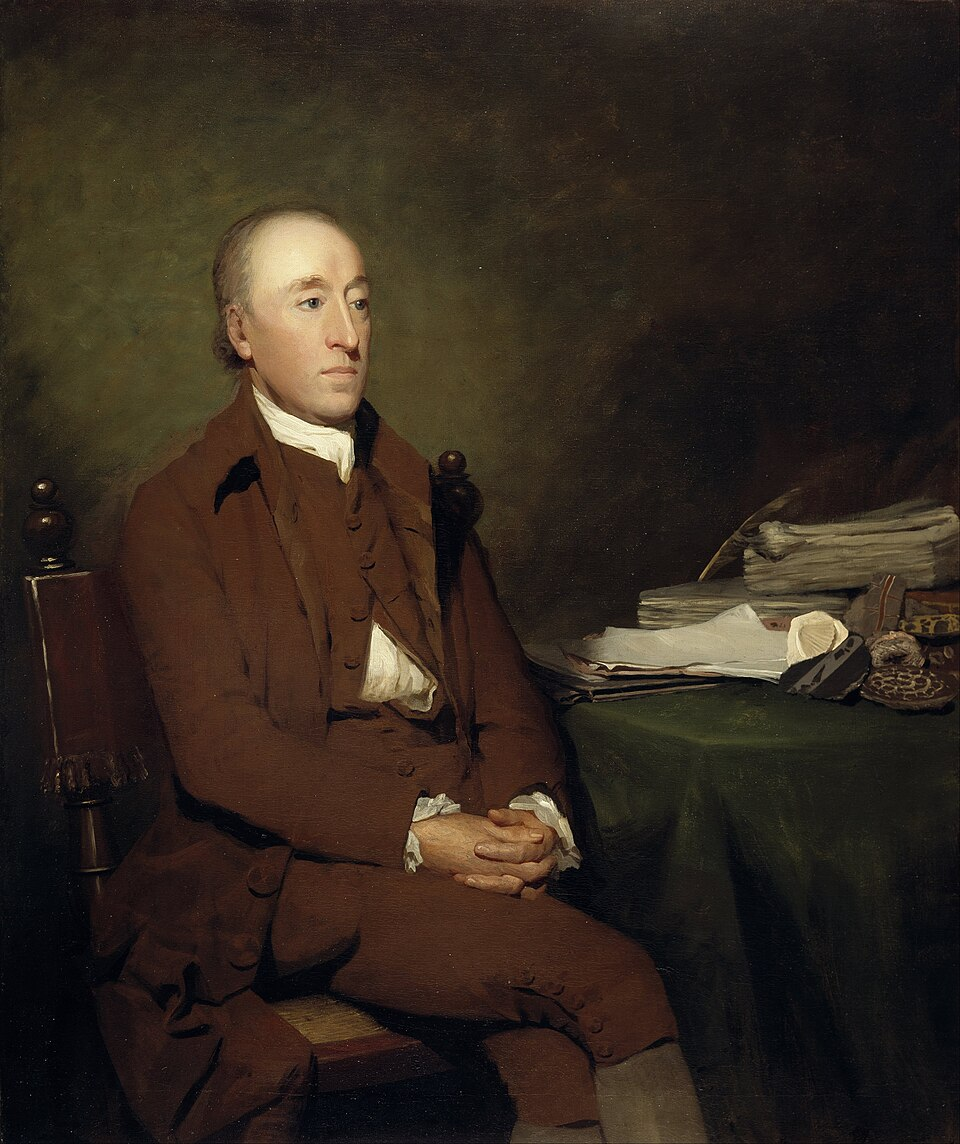
\includegraphics[width=0.3\linewidth]{images/book1/g7-hutton.jpg}

{\small James Hutton (1726--1797), peint par Henry Raeburn. Hutton
voyait dans chaque couche une durée, la plus ancienne en bas partout où
les couches n'ont pas été retournées. Portrait dans le domaine public, via
Wikimedia Commons.}
% ledger: commons:hutton-portrait, usgs:hutton-smith
\label{fig:g7:geological-time:hutton}
\end{omfigure}

Comment savoir quelle \omterm{def:g3:stones-pebbles-sand:rock}{roche} est plus ancienne qu'une autre, sans aucune
date écrite dessus~? Quel âge a la Terre~? Et comment se représenter une
si longue histoire~?

\begin{recall}
Les \omterm{def:g7:sediments-and-fossils:sediment}{sédiments} se déposent en couches, les unes sur les autres, et
durcissent en \omterm{def:g6:rocks-and-minerals:rock-families}{roches sédimentaires}~; les \omterm{def:g7:sediments-and-fossils:fossil}{fossiles} sont les restes ou les
traces d'êtres vivants conservés dans la \omterm{def:g3:stones-pebbles-sand:rock}{roche}
(\cref{ch:g7:sediments-and-fossils}). Une \emph{\omterm{def:g7:earthquakes:fault}{faille}} est une cassure
dans les \omterm{def:g3:stones-pebbles-sand:rock}{roches} le long de laquelle les deux côtés se sont déplacés
(\cref{ch:g7:earthquakes}). Le granite est une \emph{\omterm{def:g6:rocks-and-minerals:rock-families}{roche ignée}}~: il se
forme quand de la \omterm{def:g3:stones-pebbles-sand:rock}{roche} fondue refroidit lentement, en profondeur~; le
schiste est une \emph{\omterm{def:g6:rocks-and-minerals:rock-families}{roche métamorphique}}, transformée par la chaleur et
la pression~; un conglomérat est une \omterm{def:g6:rocks-and-minerals:rock-families}{roche sédimentaire} faite de \omterm{def:g3:stones-pebbles-sand:pebble}{galets}
cimentés ensemble (\cref{ch:g6:rocks-and-minerals}).
\end{recall}

\section{Qu'est-ce qui est venu d'abord~?}

Les historiens savent ranger des événements dans l'ordre même sans leurs
dates. La Première Guerre mondiale est venue avant la Seconde~: leurs
noms le disent. La télévision n'était pas encore dans les maisons quand les
frères Wright ont volé pour la première fois, en 1903, mais beaucoup de
gens ont regardé les premiers pas sur la Lune à la télévision, en 1969~:
le vol est donc venu d'abord, puis la télévision dans les maisons, puis la
Lune. Rassembler des indices et les comparer suffit pour trouver l'ordre.
Pour presque toute l'histoire de la Terre, il n'existe aucun document
écrit, et les géologues travaillent de la même façon~: ils utilisent des
indices gardés dans les \omterm{def:g3:stones-pebbles-sand:rock}{roches}.
% ledger: usgs:events-order

\begin{definition}[Datation relative et âge absolu]\label{def:g7:geological-time:relative-dating}
La \emph{datation relative}\index{datation relative} range les \omterm{def:g3:stones-pebbles-sand:rock}{roches} et
les événements dans l'ordre, du plus ancien au plus récent, sans dire il y
a combien d'années ils se sont produits~: cette \omterm{def:g3:stones-pebbles-sand:rock}{roche} est plus ancienne
que celle-là. Un \emph{âge absolu}\index{age absolu@âge absolu} est un âge
donné en nombre d'années, par exemple «~\num{300}~millions d'années~».
\end{definition}

\section{Quatre principes pour ranger les roches dans l'ordre}

Quatre principes simples font l'essentiel du travail de la \omterm{def:g7:geological-time:relative-dating}{datation
relative}. Ils sont illustrés ci-dessous, sur quatre falaises imaginaires.
Le premier a été énoncé par Nicolas Sténon en 1669~; Hutton s'en est servi à la fin du
\textsc{xviii}\textsuperscript{e}~siècle.
% ledger: usgs:hutton-smith, og:stratigraphy-principles

\begin{omfigure}
\tikzset{
  trilo/.pic={\fill[black!65] (0,0) ellipse (0.13 and 0.085);
              \draw[white, line width=0.3pt] (-0.11,0.028) -- (0.11,0.028) (-0.11,-0.028) -- (0.11,-0.028);},
  ammo/.pic={\draw[black!75, line width=0.45pt] (0,0) circle (0.1) (0,0) circle (0.062) (0,0) circle (0.028);}
}
\begin{minipage}[t]{0.49\linewidth}\centering
\begin{tikzpicture}[font=\footnotesize]
  \fill[lith sandstone] (0,0) rectangle (4.4,0.6);
  \fill[lith shale] (0,0.6) rectangle (4.4,1.2);
  \fill[lith limestone] (0,1.2) rectangle (4.4,1.8);
  \fill[lith sandstone] (0,1.8) rectangle (4.4,2.4);
  \foreach \k in {1,2,3,4} \node[fill=white, inner sep=1pt] at (0.35,0.6*\k-0.3) {\k};
  \draw (0,0) rectangle (4.4,2.4);
  \foreach \y in {0.6,1.2,1.8} \draw[contact] (0,\y) -- (4.4,\y);
  \draw[-{Stealth}, line width=0.8pt] (4.75,0.1) -- (4.75,2.3);
  \node[anchor=west] at (4.85,2.2) {la plus récente};
  \node[anchor=west] at (4.85,0.2) {la plus ancienne};
\end{tikzpicture}

{\small (a) Superposition~: la couche 1 s'est formée la première, la couche 4 la dernière.}
\end{minipage}\hfill
\begin{minipage}[t]{0.49\linewidth}\centering
\begin{tikzpicture}[font=\footnotesize]
  % left block, below the fault
  \begin{scope}
    \clip (0,0) -- (3.75,0) -- (3.25,2.4) -- (0,2.4) -- cycle;
    \fill[lith sandstone] (0,0) rectangle (5,0.6);
    \fill[lith shale] (0,0.6) rectangle (5,1.2);
    \fill[lith limestone] (0,1.2) rectangle (5,1.8);
    \fill[lith granite] (1.2,0) -- (1.85,0) -- (1.75,0.9) -- (1.9,1.8) -- (1.15,1.8) -- (1.3,0.9) -- cycle;
    \fill[lith sandstone] (0,1.8) rectangle (5,2.4);
    \foreach \y in {0.6,1.2} {\draw[contact] (0,\y) -- (1.25,\y); \draw[contact] (1.8,\y) -- (5,\y);}
    \draw[contact] (1.2,0) -- (1.3,0.9) -- (1.15,1.8) (1.85,0) -- (1.75,0.9) -- (1.9,1.8);
    \draw[contact] (0,1.8) -- (5,1.8);
  \end{scope}
  % right block, moved down along the fault
  \begin{scope}
    \clip (3.75,0) -- (5,0) -- (5,2.05) -- (3.32,2.05) -- cycle;
    \fill[lith sandstone] (3,-0.35) rectangle (5,0.25);
    \fill[lith shale] (3,0.25) rectangle (5,0.85);
    \fill[lith limestone] (3,0.85) rectangle (5,1.45);
    \fill[lith sandstone] (3,1.45) rectangle (5,2.05);
    \foreach \y in {0.25,0.85,1.45} \draw[contact] (3,\y) -- (5,\y);
  \end{scope}
  \draw (0,0) -- (5,0) -- (5,2.05) -- (3.32,2.05) (3.25,2.4) -- (0,2.4) -- (0,0);
  \draw[fault] (3.75,0) -- (3.25,2.4);
  \node[anchor=south, fill=white, inner sep=1pt] at (1.5,2.45) {granite};
  \draw[black!70] (1.5,2.45) -- (1.52,1.6);
  \node[anchor=south] at (4.2,2.45) {faille};
  \draw[black!70] (4.0,2.45) -- (3.4,1.75);
\end{tikzpicture}

{\small (b) Recoupement~: le granite est plus récent que les trois couches
qu'il recoupe, et plus ancien que la couche du haut~; la \omterm{def:g7:earthquakes:fault}{faille}, qui les
casse toutes, est la plus récente.}
\end{minipage}

\bigskip
\begin{minipage}[t]{0.49\linewidth}\centering
\begin{tikzpicture}[font=\footnotesize]
  \fill[lith granite] (0,0) -- (4.4,0) -- (4.4,1.05) .. controls (3.4,0.95) and (2.6,1.2) .. (1.6,1.0) .. controls (0.9,0.88) and (0.4,1.1) .. (0,1.0) -- cycle;
  \fill[lith conglomerate] (0,2.4) -- (4.4,2.4) -- (4.4,1.05) .. controls (3.4,0.95) and (2.6,1.2) .. (1.6,1.0) .. controls (0.9,0.88) and (0.4,1.1) .. (0,1.0) -- cycle;
  \foreach \x/\y/\a/\b in {0.5/1.35/0.2/0.12, 1.3/1.25/0.16/0.1, 2.1/1.45/0.22/0.13, 2.9/1.3/0.17/0.11, 3.7/1.4/0.2/0.12, 0.9/1.8/0.15/0.1, 2.5/1.95/0.17/0.1, 3.4/1.85/0.14/0.09}
    \filldraw[fill=omLithGranite, draw=black!70, line width=0.3pt] (\x,\y) ellipse [x radius=\a, y radius=\b];
  \draw[unconformity] (0,1.0) .. controls (0.4,1.1) and (0.9,0.88) .. (1.6,1.0) .. controls (2.6,1.2) and (3.4,0.95) .. (4.4,1.05);
  \draw (0,0) rectangle (4.4,2.4);
  \node[fill=white, inner sep=1pt] at (2.2,0.45) {granite};
  \node[anchor=west] at (4.5,1.7) {conglomérat};
  \node[anchor=west, align=left] at (4.5,1.15) {galets de\\granite};
  \draw[black!70] (4.5,1.15) -- (3.85,1.4);
\end{tikzpicture}

{\small (c) Inclusion~: les \omterm{def:g3:stones-pebbles-sand:pebble}{galets} de granite sont plus anciens que le
conglomérat qui les contient.}
\end{minipage}\hfill
\begin{minipage}[t]{0.49\linewidth}\centering
\begin{tikzpicture}[font=\footnotesize]
  % place A
  \fill[lith shale] (0,0) rectangle (1.3,0.8);
  \fill[lith limestone] (0,0.8) rectangle (1.3,1.6);
  \fill[lith sandstone] (0,1.6) rectangle (1.3,2.4);
  \draw (0,0) rectangle (1.3,2.4); \draw[contact] (0,0.8) -- (1.3,0.8) (0,1.6) -- (1.3,1.6);
  \foreach \x in {0.3,0.65,1.0} {\pic at (\x,0.4) {trilo}; \pic at (\x,1.2) {ammo};}
  \node[anchor=south] at (0.65,2.45) {lieu A};
  % place B
  \fill[lith sandstone] (3.6,0.4) rectangle (4.9,1.0);
  \fill[lith shale] (3.6,1.0) rectangle (4.9,2.0);
  \fill[lith limestone] (3.6,0) rectangle (4.9,0.4);
  \draw (3.6,0) rectangle (4.9,2.0); \draw[contact] (3.6,0.4) -- (4.9,0.4) (3.6,1.0) -- (4.9,1.0);
  \foreach \x in {3.9,4.25,4.6} {\pic at (\x,0.7) {trilo}; \pic at (\x,1.5) {ammo};}
  \node[anchor=south] at (4.25,2.45) {lieu B};
  \draw[dashed, black!70] (1.3,0.8) -- (3.6,1.0) (1.3,0) -- (3.6,0.4) (1.3,1.6) -- (3.6,2.0);
  \pic at (2.15,-0.3) {trilo}; \node[anchor=west] at (2.3,-0.3) {trilobite};
  \pic at (2.15,2.3) {ammo}; \node[anchor=west] at (2.3,2.3) {ammonite};
\end{tikzpicture}

{\small (d) Identité paléontologique~: les couches qui contiennent les
mêmes \omterm{def:g7:sediments-and-fossils:fossil}{fossiles} ont le même âge, même si leurs \omterm{def:g3:stones-pebbles-sand:rock}{roches} diffèrent.}
\end{minipage}

\medskip
{\small Les quatre principes de la \omterm{def:g7:geological-time:relative-dating}{datation relative}, sur quatre falaises
imaginaires.}
% ledger: usgs:hutton-smith, usgs:cross-cutting, nps:cross-cutting, eli:relative-dating, usgs:fossil-succession
\label{fig:g7:geological-time:principles}
\end{omfigure}

\begin{definition}[Principe de superposition]\label{def:g7:geological-time:superposition}
Le \emph{principe de superposition}\index{superposition, principe de}~:
dans une pile de \omterm{def:g7:sediments-and-fossils:layer}{couches sédimentaires} qui n'a pas été retournée, chaque
couche est plus récente que la couche située au-dessous et plus ancienne
que la couche située au-dessus. La couche la plus ancienne est en bas, la
plus récente en haut.
\end{definition}
% ledger: usgs:hutton-smith, eli:relative-dating

\begin{definition}[Principe de recoupement]\label{def:g7:geological-time:cross-cutting}
Le \emph{principe de recoupement}\index{recoupement, principe de}~: une
\omterm{def:g3:stones-pebbles-sand:rock}{roche} ou une structure qui recoupe d'autres \omterm{def:g3:stones-pebbles-sand:rock}{roches} est plus récente que
les \omterm{def:g3:stones-pebbles-sand:rock}{roches} qu'elle recoupe. Une masse de granite qui traverse des couches,
une \omterm{def:g7:earthquakes:fault}{faille} qui les casse et une surface d'\omterm{def:g5:water-shapes-the-land:erosion}{érosion} qui les use sont toutes
plus récentes que ces couches.
\end{definition}
% ledger: usgs:cross-cutting, nps:cross-cutting, eli:relative-dating

\begin{definition}[Principe d'inclusion]\label{def:g7:geological-time:inclusion}
Le \emph{principe d'inclusion}\index{inclusion, principe d'}~: des morceaux
d'une \omterm{def:g3:stones-pebbles-sand:rock}{roche} trouvés à l'intérieur d'une autre \omterm{def:g3:stones-pebbles-sand:rock}{roche} sont plus anciens que
la \omterm{def:g3:stones-pebbles-sand:rock}{roche} qui les contient. Les \omterm{def:g3:stones-pebbles-sand:pebble}{galets} d'un conglomérat existaient avant
que le conglomérat ne se forme autour d'eux.
\end{definition}
% ledger: eli:relative-dating

\begin{definition}[Principe d'identité paléontologique]\label{def:g7:geological-time:fossil-succession}
Le \emph{principe d'identité paléontologique}\index{identite paleontologique, principe d'@identité paléontologique, principe d'}~: les sortes
d'animaux et de plantes que l'on trouve à l'état \omterm{def:g7:sediments-and-fossils:fossil}{fossile} changent des
couches les plus anciennes aux plus récentes, toujours dans le même
ordre. Des \omterm{def:g3:stones-pebbles-sand:rock}{roches} qui contiennent les mêmes sortes de \omterm{def:g7:sediments-and-fossils:fossil}{fossiles} ont le même
âge, même quand elles sont très éloignées l'une de l'autre.
\end{definition}
% ledger: usgs:fossil-succession


Le \omterm{def:g7:geological-time:superposition}{principe de superposition} ne vaut que pour des couches qui n'ont pas
été retournées~: en quelques endroits, la formation des \omterm{def:g1:landscapes-around-us:landform}{montagnes} a plissé
une pile de couches si fortement qu'elle se retrouve à l'envers. Les
géologues cherchent alors des indices qui montrent dans quel sens les
couches se sont formées --- les empreintes de pas et les rides de
courant, par exemple, se trouvent à la surface du haut d'une couche. Le
\omterm{def:g7:geological-time:fossil-succession}{principe d'identité paléontologique} fonctionne parce que la vie sur Terre
a changé au cours du temps~: la plupart des \omterm{def:g7:sediments-and-fossils:fossil}{fossiles} appartiennent à des
espèces qui ne vivent plus nulle part. Pourquoi la vie a changé, les
livres de biologie le racontent.
% ledger: eli:relative-dating, usgs:fossil-succession, nps:ripple-marks

\begin{history}[William Smith, le bâtisseur de canaux]
Entre 1785 et 1800, pendant que Hutton travaillait en Écosse, William
Smith, un ingénieur anglais qui construisait des canaux, recueillit les
coquilles \omterm{def:g7:sediments-and-fossils:fossil}{fossiles} des calcaires et des argilites qu'il creusait. Il
découvrit que chaque couche avait ses propres \omterm{def:g7:sediments-and-fossils:fossil}{fossiles}, différents de ceux
des couches situées au-dessus et au-dessous. En se servant de ces
\omterm{def:g7:sediments-and-fossils:fossil}{fossiles} comme de repères, il pouvait reconnaître la même couche partout
où elle apparaissait, et il dessina certaines des premières \omterm{def:g2:drawing-to-map:map}{cartes}
géologiques de vastes régions.
\end{history}
% ledger: usgs:hutton-smith

\section{Des lacunes dans les archives}

À Siccar Point, les couches grises et le grès rouge ne se sont pas formés
l'un après l'autre. Entre les deux, les couches grises ont été inclinées
et soulevées, puis usées pendant très longtemps, et aucune couche de cette
époque n'a été conservée. La surface entre les deux ensembles de \omterm{def:g3:stones-pebbles-sand:rock}{roches}
est une lacune dans les archives de la Terre.

\begin{definition}[Discordance]\label{def:g7:geological-time:unconformity}
Une \emph{discordance}\index{discordance} est une surface d'\omterm{def:g5:water-shapes-the-land:erosion}{érosion} entre
deux ensembles de \omterm{def:g3:stones-pebbles-sand:rock}{roches} formés à des époques très différentes~: les
\omterm{def:g3:stones-pebbles-sand:rock}{roches} les plus anciennes ont été usées avant que les plus récentes ne se
déposent par-dessus. Elle marque une longue durée dont aucune couche n'a
été conservée.
\end{definition}
% ledger: ncse:siccar-point, eli:relative-dating

\begin{omfigure}
\begin{tikzpicture}[font=\footnotesize, x=1cm, y=1cm]
  \def\stripes#1#2#3{% x0, width, top: vertical layers
    \foreach \i in {0,...,7} {
      \pgfmathsetmacro{\xa}{#1+\i*#2/8}
      \pgfmathsetmacro{\xb}{#1+(\i+1)*#2/8}
      \ifodd\i\def\lithc{omLithSchist}\else\def\lithc{omLithShale}\fi
      \fill[\lithc] (\xa,0) rectangle (\xb,#3);
      \draw[black!55, line width=0.3pt] (\xa,0) -- (\xa,#3);
    }}
  % 1: flat layers under the sea
  \fill[omSea!70] (0,1.6) rectangle (3.4,2.4);
  \foreach \k in {0,...,3} {
    \ifodd\k\def\lithc{omLithSchist}\else\def\lithc{omLithShale}\fi
    \fill[\lithc] (0,0.4*\k) rectangle (3.4,0.4*\k+0.4);
    \draw[black!55, line width=0.3pt] (0,0.4*\k) -- (3.4,0.4*\k);
  }
  \draw (0,0) rectangle (3.4,2.4);
  \node[anchor=north, align=center] at (1.7,-0.1) {1. Couches déposées\\à plat dans une mer};
  % 2: pushed up on end
  \begin{scope}[xshift=3.9cm]
    \begin{scope}
      \clip (0,0) -- (3.4,0) -- (3.4,1.7) -- (2.6,2.2) -- (1.6,1.75) -- (0.9,2.3) -- (0,1.8) -- cycle;
      \stripes{0}{3.4}{2.4}
    \end{scope}
    \draw (0,1.8) -- (0.9,2.3) -- (1.6,1.75) -- (2.6,2.2) -- (3.4,1.7);
    \draw (0,1.8) -- (0,0) -- (3.4,0) -- (3.4,1.7);
    \node[anchor=north, align=center] at (1.7,-0.1) {2. Redressées,\\soulevées hors de la mer};
  \end{scope}
  % 3: worn flat
  \begin{scope}[xshift=7.8cm]
    \stripes{0}{3.4}{1.3}
    \draw[unconformity] (0,1.3) -- (3.4,1.3);
    \draw (0,1.3) -- (0,0) -- (3.4,0) -- (3.4,1.3);
    \node[anchor=north, align=center] at (1.7,-0.1) {3. Usées pendant\\longtemps};
  \end{scope}
  % 4: new layers on top
  \begin{scope}[xshift=11.7cm]
    \stripes{0}{3.4}{1.3}
    \fill[om lith={red!22}{om sand}] (0,1.3) rectangle (3.4,1.85);
    \fill[om lith={red!30}{om sand}] (0,1.85) rectangle (3.4,2.4);
    \draw[contact] (0,1.85) -- (3.4,1.85);
    \draw[unconformity, line width=0.9pt] (0,1.3) -- (3.4,1.3);
    \draw (0,0) rectangle (3.4,2.4);
    \node[anchor=north, align=center] at (1.7,-0.1) {4. De nouvelles couches\\par-dessus~: une discordance};
  \end{scope}
  \foreach \x in {3.45,7.35,11.25} \draw[-{Stealth}, line width=0.7pt] (\x,1.2) -- (\x+0.4,1.2);
\end{tikzpicture}

{\small Comment se forme une \omterm{def:g7:geological-time:unconformity}{discordance} comme celle de Siccar Point. La
ligne ondulée est la \omterm{def:g7:geological-time:unconformity}{discordance}~: la longue durée des étapes 2 et 3 n'a
laissé aucune couche.}
% ledger: ncse:siccar-point
\label{fig:g7:geological-time:unconformity}
\end{omfigure}

\section{Lire l'histoire d'une région}

Une coupe montre les \omterm{def:g3:stones-pebbles-sand:rock}{roches} telles qu'elles apparaîtraient dans une
tranchée creusée verticalement dans le sol. Les quatre principes la
changent en récit.

\begin{method}[Ranger dans l'ordre les événements d'une coupe]\label{met:g7:geological-time:ordering}
\begin{enumerate}
  \item Trouve les \omterm{def:g3:stones-pebbles-sand:rock}{roches} les plus anciennes~: celles que tout le reste
        recoupe, ou qui sont au bas de la pile.
  \item Trouve chaque \omterm{def:g3:stones-pebbles-sand:rock}{roche} ou structure qui en recoupe d'autres (un
        granite, une \omterm{def:g7:earthquakes:fault}{faille}, une surface d'\omterm{def:g5:water-shapes-the-land:erosion}{érosion})~: elle est plus
        récente que tout ce qu'elle recoupe.
  \item Lis les couches de bas en haut (superposition), et cherche les
        \omterm{def:g7:geological-time:unconformity}{discordances}, là où du temps manque.
  \item Les couches se déposent à plat~: si elles sont inclinées ou
        plissées, le plissement est venu après elles.
  \item Écris les événements dans l'ordre, du plus ancien au plus récent,
        avec l'indice de chacun.
\end{enumerate}
\end{method}
% ledger: eli:relative-dating, usgs:cross-cutting, nps:cross-cutting

\begin{omfigure}
\begin{tikzpicture}
\begin{axis}[x=1.4cm, y=0.007cm, xmin=0, xmax=10, ymin=-500, ymax=300,
  axis on top, tick label style={font=\scriptsize}, label style={font=\small},
  xlabel={distance à l'est de E (km)}, ylabel={altitude (m)},
  ytick={-400,-200,0,200}, clip mode=individual]
\addplot[lith schist, draw=black, line width=0.3pt, even odd rule] table {figdata/out/grade-7-varden_history-unit-schist.dat};
\addplot[lith granite, draw=black, line width=0.3pt, even odd rule] table {figdata/out/grade-7-varden_history-unit-granite.dat};
\addplot[om lith={icsTriassic!35}{om sand}, draw=black, line width=0.3pt, even odd rule] table {figdata/out/grade-7-varden_history-unit-sandstone.dat};
\addplot[om lith={icsJurassic!40}{om limestone}, draw=black, line width=0.3pt, even odd rule] table {figdata/out/grade-7-varden_history-unit-limestone.dat};
\addplot[om lith={icsJurassic!15}{om shale}, draw=black, line width=0.3pt, even odd rule] table {figdata/out/grade-7-varden_history-unit-shale.dat};
\addplot[om lith={icsCretaceous!35}{om limestone}, draw=black, line width=0.3pt, even odd rule] table {figdata/out/grade-7-varden_history-unit-chalk.dat};
\addplot[lith alluvium, draw=black, line width=0.3pt, even odd rule] table {figdata/out/grade-7-varden_history-unit-alluvium.dat};
\addplot[omThm, line width=1.3pt] table {figdata/out/grade-7-varden_history-base.dat};
\addplot[black, line width=0.8pt] table {figdata/out/grade-7-varden_history-ground.dat};
\addplot[fault, line width=1.3pt] table {figdata/out/grade-7-varden_history-fault.dat};
\node[font=\small, above right] at (axis cs:0,300) {E (ouest)};
\node[font=\small, above left] at (axis cs:10,300) {F (est)};
\end{axis}
\end{tikzpicture}

\smallskip
{\small\setlength{\tabcolsep}{4pt}
\begin{tabular}{@{}llll@{}}
\tikz\fill[lith schist, draw=black] (0,0) rectangle (0.5,0.3); schiste &
\tikz\fill[lith granite, draw=black] (0,0) rectangle (0.5,0.3); granite &
\tikz\fill[om lith={icsTriassic!35}{om sand}, draw=black] (0,0) rectangle (0.5,0.3); grès &
\tikz\fill[om lith={icsJurassic!40}{om limestone}, draw=black] (0,0) rectangle (0.5,0.3); calcaire \\
\tikz\fill[om lith={icsJurassic!15}{om shale}, draw=black] (0,0) rectangle (0.5,0.3); argilite &
\tikz\fill[om lith={icsCretaceous!35}{om limestone}, draw=black] (0,0) rectangle (0.5,0.3); craie &
\tikz\fill[lith alluvium, draw=black] (0,0) rectangle (0.5,0.3); \omterm{def:g3:stones-pebbles-sand:sand}{sable} de \omterm{def:g1:landscapes-around-us:water}{rivière} &
\tikz\draw[omThm, line width=1.3pt] (0,0.15) -- (0.5,0.15); base du grès \\
\end{tabular}}

\smallskip
{\small Coupe E--F, d'ouest (E) en est (F), à travers le milieu des
collines de Varden, la région inventée de cette collection, en passant par
son granite. Le gros trait noir est la \omterm{def:g7:earthquakes:fault}{faille}. Les hauteurs sont étirées
5~fois par rapport aux distances, pour que les couches se voient mieux.}
% ledger: (invented region: figdata/shared/region.py, section E--F by figdata/grade-7/varden_history.py)
\label{fig:g7:geological-time:section}
\end{omfigure}

\begin{example}[L'histoire des collines de Varden]\label{ex:g7:geological-time:varden}
Appliquons la méthode à la coupe E--F.
\begin{enumerate}
  \item Le schiste est recoupé par le granite et se trouve sous toutes les
        couches~: c'est la \omterm{def:g3:stones-pebbles-sand:rock}{roche} la plus ancienne.
  \item Le granite recoupe le schiste (recoupement)~: il est donc plus
        récent. Il ne recoupe aucune des couches du dessus~: il est plus
        ancien que le grès.
  \item Le granite a refroidi en profondeur, et pourtant la base du grès,
        qui repose sur le schiste, atteint le sommet du granite~: les
        \omterm{def:g3:stones-pebbles-sand:rock}{roches} qui les recouvraient ont été usées avant l'arrivée du
        \omterm{def:g3:stones-pebbles-sand:sand}{sable}. La base du grès est une \omterm{def:g7:geological-time:unconformity}{discordance}.
  \item Le grès, le calcaire, l'argilite et la craie se sont déposés dans
        cet ordre (superposition).
  \item Les couches se sont déposées à plat, mais elles sont aujourd'hui
        plissées, bombées au-dessus du granite et courbées vers le bas plus
        à l'est~: le plissement est venu après la craie.
  \item La \omterm{def:g7:earthquakes:fault}{faille} casse toutes les couches plissées~: elle est plus
        récente que le plissement.
  \item La surface actuelle du sol recoupe tout, et le \omterm{def:g3:stones-pebbles-sand:sand}{sable} de \omterm{def:g1:landscapes-around-us:water}{rivière}
        repose sur elle~: l'\omterm{def:g5:water-shapes-the-land:erosion}{érosion} et les \omterm{def:g1:landscapes-around-us:water}{rivières} sont les événements les
        plus récents.
\end{enumerate}
L'histoire, du plus ancien au plus récent~: le schiste~; le granite~;
l'\omterm{def:g5:water-shapes-the-land:erosion}{érosion}~; les quatre couches~; le plissement~; la \omterm{def:g7:earthquakes:fault}{faille}~; l'\omterm{def:g5:water-shapes-the-land:erosion}{érosion}
actuelle et le \omterm{def:g3:stones-pebbles-sand:sand}{sable} de \omterm{def:g1:landscapes-around-us:water}{rivière}.
% ledger: (invented region: figdata/grade-7/varden_history.py main table)
\end{example}

La \omterm{def:g7:geological-time:relative-dating}{datation relative} donne l'ordre des événements, mais ni leurs dates, ni
la durée de chacun~: la méthode dit que la \omterm{def:g7:earthquakes:fault}{faille} est plus récente que la
craie, pas de combien d'années.

\section{Ères et périodes}

L'identité paléontologique permet aux géologues de faire correspondre des
couches du monde entier. En réunissant leurs observations, ils ont divisé
l'histoire de la Terre en intervalles de temps, de la même façon que les
historiens parlent de siècles et de règnes.
% ledger: usgs:hutton-smith, usgs:fossil-succession

\begin{omfigure}
\begin{tikzpicture}[font=\footnotesize]
\begin{axis}[name=long, x dir=reverse, xmin=0, xmax=4600, ymin=0, ymax=1,
  width=14.3cm, height=1.7cm, scale only axis, axis y line=none, axis x line*=bottom,
  xtick={4500,4000,3000,2000,1000}, tick label style={font=\scriptsize}, clip=false]
  \pgfplotsinvokeforeach{Hadean,Archean,Proterozoic,Phanerozoic}{
    \addplot[fill=ics#1, draw=black!70, line width=0.3pt] table {figdata/out/grade-7-time_scale-bar-#1.dat};}
  \node[anchor=center, font=\scriptsize, fill=white, fill opacity=0.85, text opacity=1, inner sep=1pt] at (axis cs:4299,0.5) {Hadéen};
  \node[anchor=center, font=\scriptsize, fill=white, fill opacity=0.85, text opacity=1, inner sep=1pt] at (axis cs:3265.5,0.5) {Archéen};
  \node[anchor=center, font=\scriptsize, fill=white, fill opacity=0.85, text opacity=1, inner sep=1pt] at (axis cs:1519.4,0.5) {Protérozoïque};
  \node[anchor=center, font=\scriptsize, fill=white, fill opacity=0.85, text opacity=1, inner sep=1pt] at (axis cs:269.4,0.5) {Phanérozoïque};
  \coordinate (z1) at (axis cs:538.8,0);
  \coordinate (z2) at (axis cs:0,0);
\end{axis}
\begin{axis}[at={(long.south west)}, anchor=north west, yshift=-1.3cm,
  x dir=reverse, xmin=0, xmax=540, ymin=0, ymax=3.2,
  width=14.3cm, height=3.6cm, scale only axis, axis y line=none, axis x line*=bottom,
  xtick={500,400,300,200,100,0}, tick label style={font=\scriptsize},
  xlabel={millions d'années avant aujourd'hui}, label style={font=\small}, clip=false]
  \pgfplotsinvokeforeach{Paleozoic,Mesozoic,Cenozoic}{
    \addplot[fill=ics#1, draw=black!70, line width=0.3pt] table[x=age, y expr=2.4+0.8*\thisrow{y}] {figdata/out/grade-7-time_scale-bar-#1.dat};}
  \pgfplotsinvokeforeach{Cambrian,Ordovician,Silurian,Devonian,Carboniferous,Permian,Triassic,Jurassic,Cretaceous,Paleogene,Neogene,Quaternary}{
    \addplot[fill=ics#1, draw=black!70, line width=0.3pt] table[x=age, y expr=2.4*\thisrow{y}] {figdata/out/grade-7-time_scale-bar-#1.dat};}
  \node[anchor=center, font=\footnotesize\bfseries, fill=white, fill opacity=0.85, text opacity=1, inner sep=1pt] at (axis cs:395.351,2.8) {Paléozoïque};
  \node[anchor=center, font=\footnotesize\bfseries, fill=white, fill opacity=0.85, text opacity=1, inner sep=1pt] at (axis cs:158.951,2.8) {Mésozoïque};
  \node[anchor=center, font=\footnotesize\bfseries, fill=white, fill opacity=0.85, text opacity=1, inner sep=1pt] at (axis cs:33,2.8) {Cénozoïque};
  \node[anchor=center, rotate=90, font=\scriptsize, fill=white, fill opacity=0.85, text opacity=1, inner sep=1pt] at (axis cs:512.825,1.2) {Cambrien};
  \node[anchor=center, rotate=90, font=\scriptsize, fill=white, fill opacity=0.85, text opacity=1, inner sep=1pt] at (axis cs:464.975,1.2) {Ordovicien};
  \node[anchor=center, rotate=90, font=\scriptsize, fill=white, fill opacity=0.85, text opacity=1, inner sep=1pt] at (axis cs:431.36,1.2) {Silurien};
  \node[anchor=center, rotate=90, font=\scriptsize, fill=white, fill opacity=0.85, text opacity=1, inner sep=1pt] at (axis cs:389.24,1.2) {Dévonien};
  \node[anchor=center, rotate=90, font=\scriptsize, fill=white, fill opacity=0.85, text opacity=1, inner sep=1pt] at (axis cs:328.88,1.2) {Carbonifère};
  \node[anchor=center, rotate=90, font=\scriptsize, fill=white, fill opacity=0.85, text opacity=1, inner sep=1pt] at (axis cs:275.401,1.2) {Permien};
  \node[anchor=center, rotate=90, font=\scriptsize, fill=white, fill opacity=0.85, text opacity=1, inner sep=1pt] at (axis cs:226.651,1.2) {Trias};
  \node[anchor=center, rotate=90, font=\scriptsize, fill=white, fill opacity=0.85, text opacity=1, inner sep=1pt] at (axis cs:172.25,1.2) {Jurassique};
  \node[anchor=center, rotate=90, font=\scriptsize, fill=white, fill opacity=0.85, text opacity=1, inner sep=1pt] at (axis cs:104.55,1.2) {Crétacé};
  \node[anchor=center, rotate=90, font=\scriptsize, fill=white, fill opacity=0.85, text opacity=1, inner sep=1pt] at (axis cs:44.52,1.2) {Paléogène};
  \node[anchor=center, rotate=90, font=\scriptsize, fill=white, fill opacity=0.85, text opacity=1, inner sep=1pt] at (axis cs:12.81,1.2) {Néogène};
  \node[anchor=west, xshift=3pt, font=\scriptsize] at (axis cs:1.29,1.2) {Quaternaire};
  \coordinate (w1) at (axis cs:540,3.2);
  \coordinate (w2) at (axis cs:0,3.2);
\end{axis}
\draw[dashed, black!60] (z1) -- ++(0,-0.5) -- (w1) (z2) -- (w2);
\end{tikzpicture}

{\small L'échelle des temps géologiques, aux couleurs de la charte
internationale. En haut~: toute l'histoire de la Terre. En bas~: sa
dernière partie, le Phanérozoïque, étirée~: ses trois \omterm{def:g7:geological-time:era-period}{ères} et les douze
\omterm{def:g7:geological-time:era-period}{périodes géologiques}. Âges en millions d'années avant aujourd'hui.}
% ledger: ics:base.Hadean, ics:base.Archean, ics:base.Proterozoic, ics:base.Paleozoic, ics:base.Mesozoic, ics:base.Cenozoic, ics:colour.Hadean (figdata/grade-7/time_scale.py reads every ics base and colour row of the shared ledger)
\label{fig:g7:geological-time:scale}
\end{omfigure}

\begin{definition}[Ère et période géologique]\label{def:g7:geological-time:era-period}
Une \emph{ère}\index{ere@ère} est un long intervalle de l'histoire de la
Terre, défini par la sorte de vie qui existait de façon générale à cette
époque~: le Paléozoïque, le Mésozoïque et le Cénozoïque. Chaque ère est
divisée en intervalles plus courts, les
\emph{périodes géologiques}\index{periode geologique@période géologique},
comme le Jurassique ou le Crétacé.
\end{definition}
% ledger: usgs:hutton-smith

\begin{definition}[Échelle des temps géologiques]\label{def:g7:geological-time:time-scale}
L'\emph{échelle des temps géologiques}\index{echelle des temps geologiques@échelle des temps géologiques}
est la liste, dans l'ordre, des divisions de l'histoire de la Terre --- les
longs intervalles de ses débuts, les \omterm{def:g7:geological-time:era-period}{ères} et les \omterm{def:g7:geological-time:era-period}{périodes géologiques} ---,
avec l'âge, en années, du début de chacune. Une charte internationale
donne à chaque division son nom, son âge et sa couleur.
\end{definition}
% ledger: ics:base.Hadean, ics:colour.Hadean


Les trois \omterm{def:g7:geological-time:era-period}{ères} sont récentes, comparées à toute l'histoire. Le Paléozoïque
a commencé il y a \num{538.8}~millions d'années, quand les \omterm{def:g7:sediments-and-fossils:fossil}{fossiles}
d'animaux à coquille sont devenus courants~; le Mésozoïque a duré d'il y a
\num{251.9} à il y a \num{66}~millions d'années~; le Cénozoïque, l'\omterm{def:g7:geological-time:era-period}{ère} dans
laquelle nous vivons, a commencé il y a \num{66}~millions d'années. Avant
le Paléozoïque s'étendent trois longs intervalles, l'Hadéen, l'Archéen et
le Protérozoïque~: ils couvrent environ 88~\% de l'histoire de la Terre,
et pourtant leurs \omterm{def:g7:sediments-and-fossils:fossil}{fossiles} sont rares. Les dinosaures ont vécu au
Mésozoïque~: ils ont dominé pendant plus de \num{100}~millions d'années,
et à la fin du Crétacé, ils avaient tous disparu.
% ledger: ics:base.Paleozoic, ics:base.Mesozoic, ics:base.Cenozoic, usgs:numeric-scale, usgs:dinosaurs-extinct (figdata/grade-7/time_scale.py main table: 88.1 %)

Les collines de Varden trouvent leur place sur cette échelle. Leur grès
date du Trias, leur calcaire et leur argilite du Jurassique, leur craie du
Crétacé~: tous appartiennent au Mésozoïque. Sur la coupe E--F, ils sont
dessinés dans des versions pâles des couleurs de la charte.
% ledger: (invented region: figdata/shared/region.py UNITS)

\section{L'histoire de la Terre en une année}

Des nombres en milliards d'années sont difficiles à se représenter.
Imagine plutôt toute l'histoire de la Terre ramassée en une seule année.
La Terre se forme le 1\textsuperscript{er}~janvier à minuit~; aujourd'hui,
c'est le dernier coup de minuit, à la fin du 31~décembre. La Terre a environ
\num{4540}~millions d'années~: un jour de cette année représente donc
$4540 \div 365$, soit environ \num{12.4}~millions d'années.
% ledger: usgs:age-earth (figdata/grade-7/earth_calendar.py)

\begin{omfigure}
\begin{tikzpicture}[font=\footnotesize]
\begin{axis}[xmin=0, xmax=365, ymin=0, ymax=1, width=15.2cm, height=0.9cm,
  scale only axis, axis y line=none, axis x line=none, clip=false]
  \addplot[ycomb, black!60, line width=0.4pt] table[x=day, y expr=1] {figdata/out/grade-7-earth_calendar-days.dat};
  \draw[black!70] (axis cs:0,0) rectangle (axis cs:365,1);
  \node[anchor=center, font=\scriptsize] at (axis cs:15.5,0.5) {janv.};
  \node[anchor=center, font=\scriptsize] at (axis cs:45,0.5) {févr.};
  \node[anchor=center, font=\scriptsize] at (axis cs:74.5,0.5) {mars};
  \node[anchor=center, font=\scriptsize] at (axis cs:105,0.5) {avr.};
  \node[anchor=center, font=\scriptsize] at (axis cs:135.5,0.5) {mai};
  \node[anchor=center, font=\scriptsize] at (axis cs:166,0.5) {juin};
  \node[anchor=center, font=\scriptsize] at (axis cs:196.5,0.5) {juil.};
  \node[anchor=center, font=\scriptsize] at (axis cs:227.5,0.5) {août};
  \node[anchor=center, font=\scriptsize] at (axis cs:258,0.5) {sept.};
  \node[anchor=center, font=\scriptsize] at (axis cs:288.5,0.5) {oct.};
  \node[anchor=center, font=\scriptsize] at (axis cs:319,0.5) {nov.};
  \node[anchor=center, font=\scriptsize] at (axis cs:349.5,0.5) {déc.};
  \addplot[only marks, mark=triangle*, mark size=2.6pt, omThm, mark options={rotate=180}]
    table[x=day, y expr=1.18] {figdata/out/grade-7-earth_calendar.dat};
  \node[anchor=west, rotate=40, xshift=2pt, yshift=4pt, font=\scriptsize] at (axis cs:0,1.18) {1\textsuperscript{er}~janvier~: la Terre se forme};
  \node[anchor=west, rotate=40, xshift=2pt, yshift=4pt, font=\scriptsize] at (axis cs:41,1.18) {11~février~: plus anciennes roches connues};
  \node[anchor=west, rotate=40, xshift=2pt, yshift=4pt, font=\scriptsize] at (axis cs:83.61,1.18) {25~mars~: plus anciens fossiles connus};
  \node[anchor=east, rotate=-40, xshift=-2pt, yshift=4pt, font=\scriptsize] at (axis cs:321.68,1.18) {18~novembre~: les coquilles deviennent courantes};
  \node[anchor=east, rotate=-40, xshift=-2pt, yshift=4pt, font=\scriptsize] at (axis cs:359.69,1.18) {26~décembre~: les dinosaures ont disparu};
\end{axis}
\end{tikzpicture}

{\small L'histoire de la Terre sous la forme d'une année du calendrier~:
chaque mois représente environ \num{373}~millions d'années, chaque jour
environ \num{12.4}~millions d'années. Les dates sont calculées à partir
des âges des événements.}
% ledger: usgs:age-earth, usgs:oldest-rocks, usgs:numeric-scale, ics:base.Paleozoic, ics:base.Paleogene (figdata/grade-7/earth_calendar.py)
\label{fig:g7:geological-time:calendar}
\end{omfigure}

Les plus anciennes \omterm{def:g3:stones-pebbles-sand:rock}{roches} trouvées à ce jour arrivent le 11~février~; les
plus anciens \omterm{def:g7:sediments-and-fossils:fossil}{fossiles} connus, le 25~mars. Pendant la plus grande partie de
l'année, il n'y a pas d'animaux à coquille, et les \omterm{def:g7:sediments-and-fossils:fossil}{fossiles} sont rares.
Les animaux à coquille ne deviennent courants que le 18~novembre. Les
dinosaures, après plus de \num{100}~millions d'années de règne, ont
disparu le 26~décembre, cinq jours avant la fin de l'année. Notre propre
espèce arrive dans la dernière heure du 31~décembre~: le problème de ce
chapitre cherche à quel moment.
% ledger: usgs:oldest-rocks, usgs:numeric-scale, ics:base.Paleozoic, ics:base.Paleogene, usgs:dinosaurs-extinct, hublin:jebel-irhoud

\begin{inthelab}[Un ruban du temps]
À l'intérieur, déroule \qty{4.54}{m} de ruban de papier ou de rouleau de
caisse sur le sol d'un couloir~: à raison de \qty{1}{mm} par million
d'années, il contient toute l'histoire de la Terre. Marque le début du
Paléozoïque à \qty{54}{cm} de la fin, et la fin des dinosaures à
\qty{6.6}{cm} de la fin. Essaie ensuite de marquer toute l'histoire
humaine~: notre espèce, vieille d'environ \num{300000}~ans, occupe les
derniers \qty{0.3}{mm}, moins que l'épaisseur du trait de crayon.
\end{inthelab}
% ledger: usgs:age-earth, ics:base.Paleozoic, ics:base.Paleogene, hublin:jebel-irhoud

\section{Des âges en années}

La \omterm{def:g7:geological-time:relative-dating}{datation relative} ne peut pas dire il y a combien d'années une \omterm{def:g3:stones-pebbles-sand:rock}{roche}
s'est formée. Les \omterm{def:g7:geological-time:relative-dating}{âges absolus} sont devenus possibles avec la découverte
de la radioactivité. Certains \omterm{def:g6:rocks-and-minerals:mineral}{minéraux} contiennent des atomes radioactifs,
qui se transforment lentement en d'autres atomes à un rythme régulier, le
même en tout temps et en tout lieu~; mesurer combien se sont transformés
donne l'âge du \omterm{def:g6:rocks-and-minerals:mineral}{minéral} en années. Le fonctionnement de la radioactivité
est expliqué dans les livres de physique, et la façon dont les géologues
s'en servent est le sujet d'un volume ultérieur.
% ledger: usgs:numeric-scale, usgs:age-earth

Ces mesures ont donné son âge à la Terre~: environ \num{4.54}~milliards
d'années, connu à 1~\% près. Les plus anciennes \omterm{def:g3:stones-pebbles-sand:rock}{roches} trouvées à ce jour,
dans le nord-ouest du Canada, ont \num{4.03}~milliards d'années~; de
minuscules cristaux trouvés en Australie sont encore plus anciens, jusqu'à
environ \num{4.4}~milliards d'années. L'échelle des temps elle-même réunit
les deux sortes de datation~: une \omterm{def:g3:stones-pebbles-sand:rock}{roche} dont on peut mesurer l'âge en
années, trouvée avec des couches datées par leurs \omterm{def:g7:sediments-and-fossils:fossil}{fossiles}, donne un âge
au début ou à la fin d'une \omterm{def:g7:geological-time:era-period}{période géologique}.
% ledger: usgs:age-earth, usgs:oldest-rocks, usgs:numeric-scale

\section{Exercices}

\begin{exercise}[$\star$]\label{exo:g7:geological-time:1}
Associe chaque nom à sa définition~: superposition~; recoupement~;
inclusion~; identité paléontologique~; \omterm{def:g7:geological-time:unconformity}{discordance}. (a) Une surface
d'\omterm{def:g5:water-shapes-the-land:erosion}{érosion} entre des \omterm{def:g3:stones-pebbles-sand:rock}{roches} d'âges très différents. (b) Les \omterm{def:g3:stones-pebbles-sand:pebble}{galets} d'une
\omterm{def:g3:stones-pebbles-sand:rock}{roche} sont plus anciens que la \omterm{def:g3:stones-pebbles-sand:rock}{roche}. (c) La couche du bas d'une pile
intacte est la plus ancienne. (d) Des \omterm{def:g3:stones-pebbles-sand:rock}{roches} qui contiennent les mêmes
sortes de \omterm{def:g7:sediments-and-fossils:fossil}{fossiles} ont le même âge. (e) Une \omterm{def:g7:earthquakes:fault}{faille} est plus récente que
les couches qu'elle casse.
\end{exercise}

\begin{exercise}[$\star$]\label{exo:g7:geological-time:2}
Une falaise montre quatre couches à plat, de bas en haut~: un grès rouge,
une argilite grise, un calcaire blanc et un grès jaune. (a) Quelle couche
est la plus ancienne~? Laquelle est la plus récente~? (b) Quel principe
as-tu utilisé~? (c) Que faut-il pour que la réponse soit juste~?
\end{exercise}

\begin{exercise}[$\star$]\label{exo:g7:geological-time:3}
(a) Range les trois \omterm{def:g7:geological-time:era-period}{ères} dans l'ordre, de la plus ancienne~: Mésozoïque,
Cénozoïque, Paléozoïque. (b) Dans quelle \omterm{def:g7:geological-time:era-period}{ère} vivons-nous~? (c) Dans quelle
\omterm{def:g7:geological-time:era-period}{ère} vivaient les dinosaures~? (d) À l'aide de l'échelle des temps, donne
la \omterm{def:g7:geological-time:era-period}{période géologique} qui vient juste après le Trias, et celle qui vient
juste avant le Paléogène.
\end{exercise}

\begin{exercise}[$\star$]\label{exo:g7:geological-time:4}
Vrai ou faux~? Corrige les phrases fausses. (a) La \omterm{def:g7:geological-time:relative-dating}{datation relative} donne
l'âge d'une \omterm{def:g3:stones-pebbles-sand:rock}{roche} en années. (b) Une \omterm{def:g7:earthquakes:fault}{faille} est plus récente que les
couches qu'elle recoupe. (c) Les \omterm{def:g3:stones-pebbles-sand:pebble}{galets} d'un conglomérat sont plus récents
que le conglomérat. (d) Deux couches éloignées qui contiennent les mêmes
sortes de \omterm{def:g7:sediments-and-fossils:fossil}{fossiles} ont le même âge.
\end{exercise}

\begin{exercise}[$\star\star$]\label{exo:g7:geological-time:5}
Dans une falaise, trois couches à plat (la 1 en bas, puis la 2 et la 3)
sont recoupées par un mur de granite. Une quatrième couche repose sur la
couche 3 et sur le sommet du granite, sans être recoupée. (a) Le granite
est-il plus ancien ou plus récent que la couche 3~? Explique. (b) Est-il
plus ancien ou plus récent que la couche 4~? (c) Écris les cinq
événements dans l'ordre, du plus ancien. (d) Le granite a refroidi en
profondeur. Qu'est-il arrivé au sommet du granite avant le \omterm{def:g5:water-shapes-the-land:deposition}{dépôt} de la
couche 4~?
\end{exercise}

\begin{exercise}[$\star\star$]\label{exo:g7:geological-time:6}
Utilise les débuts des \omterm{def:g7:geological-time:era-period}{ères}~: Paléozoïque \num{538.8}, Mésozoïque
\num{251.9}, Cénozoïque \num{66}~millions d'années. (a) Combien de temps a
duré le Paléozoïque~? (b) Combien de temps a duré le Mésozoïque~? (c)
Depuis combien de temps dure le Cénozoïque~? (d) Quelle \omterm{def:g7:geological-time:era-period}{ère} est la plus
longue~? Laquelle est la plus courte~?
\end{exercise}

\begin{exercise}[$\star\star$]\label{exo:g7:geological-time:7}
La Terre a environ \num{4540}~millions d'années, et le Paléozoïque a
commencé il y a \num{538.8}~millions d'années. (a) Combien de millions
d'années se sont écoulés avant le début du Paléozoïque~? (b) Quel
pourcentage de l'histoire de la Terre cela représente-t-il~? Arrondis à
l'unité. (c) Explique pourquoi la plupart des \omterm{def:g7:sediments-and-fossils:fossil}{fossiles} trouvés par les
géologues viennent des trois dernières \omterm{def:g7:geological-time:era-period}{ères}.
\end{exercise}

\begin{exercise}[$\star\star$]\label{exo:g7:geological-time:8}
Toute l'histoire de la Terre, \num{4540}~millions d'années, est dessinée
le long d'une piste de course de \qty{100}{m}~: la ligne de départ est la
formation de la Terre, la ligne d'arrivée aujourd'hui. (a) Combien de
millions d'années chaque mètre représente-t-il~? (b) Le Paléozoïque a
commencé il y a \num{538.8}~millions d'années. À combien de mètres avant la
ligne d'arrivée se trouve-t-il~? (c) Les dinosaures avaient disparu il y a
\num{66}~millions d'années. À quelle distance avant la ligne d'arrivée~?
(d) Notre espèce est apparue il y a environ \num{300000}~ans. Donne la
distance en centimètres. Un coureur pourrait-il la voir~?
\end{exercise}

\begin{exercise}[$\star\star$]\label{exo:g7:geological-time:9}
À Siccar Point, les couches grises dressées se sont formées au
Silurien~; le grès rouge qui les surmonte s'est formé au Dévonien. (a) À
l'aide de l'échelle des temps, quelle période est venue d'abord~? Est-ce
en accord avec la superposition~? (b) Range ces événements dans l'ordre~:
le \omterm{def:g3:stones-pebbles-sand:sand}{sable} rouge se dépose~; les couches grises se déposent à plat~; les
couches grises sont usées~; les couches grises sont redressées. (c)
Pourquoi la surface entre les deux \omterm{def:g3:stones-pebbles-sand:rock}{roches} s'appelle-t-elle une
\omterm{def:g7:geological-time:unconformity}{discordance}~?
\end{exercise}

\begin{exercise}[$\star\star$]\label{exo:g7:geological-time:10}
Deux falaises sont à \qty{50}{km} l'une de l'autre. La falaise A montre,
de bas en haut~: un grès à trilobites, une argilite à ammonites, un
calcaire à oursins. La falaise B montre, de bas en haut~: une argilite à
ammonites, un calcaire à oursins, une argile à feuilles. (a) Quelles
couches des deux falaises ont le même âge~? Quel principe utilises-tu~?
(b) Quelle couche est la plus ancienne de toutes~? Laquelle est la plus
récente~? (c) Dessine une seule colonne avec toutes les couches des deux
falaises, dans l'ordre.
\end{exercise}

\begin{exercise}[$\star\star\star$]\label{exo:g7:geological-time:11}
Une coupe montre~: en bas, un schiste~; sur lui, séparé par une surface
d'\omterm{def:g5:water-shapes-the-land:erosion}{érosion} ondulée, un conglomérat dont les \omterm{def:g3:stones-pebbles-sand:pebble}{galets} sont des morceaux de
schiste~; au-dessus, un grès, puis un calcaire, tous trois inclinés~; une
\omterm{def:g7:earthquakes:fault}{faille} qui casse le schiste, le conglomérat, le grès et le calcaire~; et
au sommet, des couches d'argile à plat qui recouvrent les couches
inclinées et la \omterm{def:g7:earthquakes:fault}{faille} sans être cassées. (a) Qu'est-ce qui est le plus
ancien, le schiste ou le conglomérat~? Donne deux indices. (b)
L'inclinaison a-t-elle eu lieu avant ou après le \omterm{def:g5:water-shapes-the-land:deposition}{dépôt} du grès~? (c) La
\omterm{def:g7:earthquakes:fault}{faille} est-elle venue avant ou après l'argile~? (d) Écris toute l'histoire
dans l'ordre, à partir de l'événement le plus ancien. (e) Combien y a-t-il
de \omterm{def:g7:geological-time:unconformity}{discordances}~? Où~?
\end{exercise}

\begin{exercise}[$\star\star\star$]\label{exo:g7:geological-time:12}
Utilise l'année de la Terre (\num{4540}~millions d'années en 365~jours).
(a) Quel jour l'histoire de la Terre est-elle à moitié écoulée~? Donne la
date et l'heure. (b) Quel âge, en millions d'années, a une \omterm{def:g3:stones-pebbles-sand:rock}{roche} formée à
cette date~? (c) Une année compte $365 \times 24 \times 60 \times 60 = \num{31536000}$
secondes. Une personne vit 80~ans. Combien de secondes de l'année de la
Terre cette vie dure-t-elle~? Utilise $80 \div \num{4540000000} \times
\num{31536000}$, et arrondis au dixième.
\end{exercise}

\section{Problème~: L'année de la Terre}

\begin{problem}[{Problème du week-end --- l'histoire de la Terre est
ramassée en une année du calendrier, ses grands événements sont placés à
leur date, et l'on cherche notre espèce dans les dernières minutes du
31~décembre}]
\label{pb:g7:geological-time:1}
% ledger: usgs:age-earth, usgs:oldest-rocks, usgs:numeric-scale, ics:base.Paleogene, hublin:jebel-irhoud (figdata/grade-7/earth_calendar.py)
La Terre a environ \num{4540}~millions d'années. Toute son histoire est
ramassée en une année de 365~jours, du 1\textsuperscript{er}~janvier à
minuit au 31~décembre à minuit, qui représente aujourd'hui.

\medskip
\noindent\textbf{Partie I --- Mettre le temps à l'échelle.}\par\nopagebreak
\begin{enumerate}[beginpenalty=10000]
  \item Écris \num{4.54}~milliards d'années en millions d'années.
  \item Combien de millions d'années un jour de l'année de la Terre
        représente-t-il~? Arrondis au dixième.
  \item Combien d'années une heure représente-t-elle~? Arrondis au millier
        d'années.
  \item Une année compte $365 \times 24 \times 60 = \num{525600}$ minutes.
        Combien d'années une minute représente-t-elle~? Arrondis à la
        centaine d'années.
\end{enumerate}

\medskip
\noindent\textbf{Partie II --- Placer les événements.}\par\nopagebreak
\begin{enumerate}[resume, beginpenalty=10000]
  \item Les plus anciennes \omterm{def:g3:stones-pebbles-sand:rock}{roches} trouvées à ce jour ont \num{4030}~millions
        d'années. Combien de millions d'années après la formation de la
        Terre se sont-elles formées~? Environ combien de jours de l'année
        de la Terre cela fait-il~? Donne la date.
  \item Les plus anciens \omterm{def:g7:sediments-and-fossils:fossil}{fossiles} connus ont environ \num{3500}~millions
        d'années. Trouve leur date de la même façon.
  \item Les dinosaures avaient disparu il y a \num{66}~millions d'années.
        Combien de jours avant la fin de l'année cela fait-il~? Donne la
        date.
  \item Le Paléozoïque a commencé il y a \num{538.8}~millions d'années.
        Quel pourcentage de l'année reste-t-il après son début~? En quel
        mois commence-t-il~?
\end{enumerate}

\medskip
\noindent\textbf{Partie III --- Les dernières minutes.}\par\nopagebreak
\begin{enumerate}[resume, beginpenalty=10000]
  \item À l'aide de la question 4, combien de minutes représentent
        \num{10000}~ans~? Arrondis au dixième.
  \item Suppose que l'écriture a été inventée il y a environ \num{5000}~ans.
        Combien de secondes avant minuit, le 31~décembre, apparaît-elle~?
  \item Notre espèce, \emph{Homo sapiens}, est apparue il y a environ
        \num{300000}~ans. Combien de minutes avant minuit cela fait-il~?
        Arrondis à la minute.
  \item À quelle heure, le 31~décembre, notre espèce apparaît-elle~?
\end{enumerate}
\end{problem}
